%\newpage

%% \section{Appendix: Real DNN versus HT Random Matrices}
%% \label{sxn:appendix-dnn_versus_random}
%% 
%% \michael{MM still to fix this.}
%% 
%% \paragraph{Properties of our Basic Relation of Eqn.~(\ref{eqn:basic_relation}).}
%% XXX.  MAYBE PUT THIS IN APPENDIX.
%% 
%% \charlesX{
%% TODO:  explain plots.
%% Refer to Figure~\ref{fig:relations}.
%% 
%% Multiplying $\alpha$ by $\log_{10}\lambda_{max}$, we now have a relation that increases nearly linearly with the Frobenius norm for a random matrix, and is linearly correlated for real DNN data. Which is exactly what we want for our simple complexity metric.
%% 
%% Note that while linear relation holds over several log scales, 
%% the relation does deviate from linearity at the smaller values of $\alpha\;\log_{10}\;\lambda_{max}$.
%% This is readily explained below .  
%% XXX.  WHAT FIG ARE WE REFERRING TO, PRESUMABLY FIG~\ref{fig:relation-vgg11}.
%% }
%% 
%%  \begin{figure}[t] %[!htb]
%%     \centering
%%    \subfigure[Random Pareto Matrices] {
%%        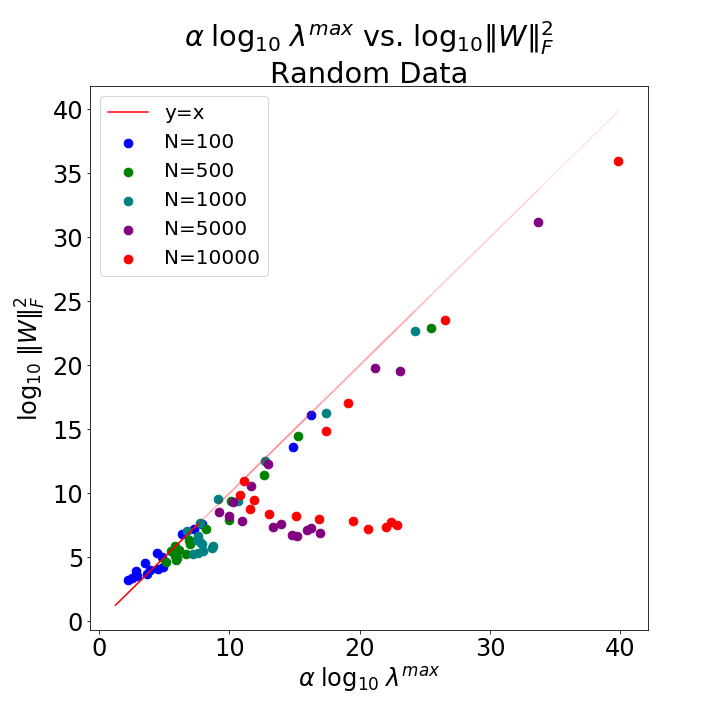
\includegraphics[scale=0.30]{img/relation-rand.png} 
%%        \label{fig:relation-rand}
%%    }
%%    \subfigure[VGG 11 Weight matrices]{
%%        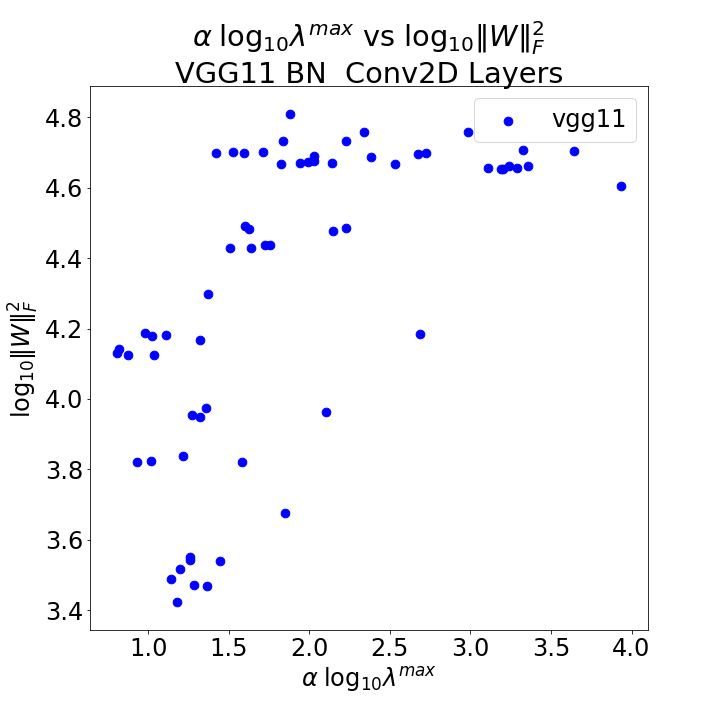
\includegraphics[scale=0.30]{img/relation-vgg11.png} 
%%        \label{fig:relation-vgg11}
%%    }
%%        \caption{Relation between $\alpha\;\log_{10}\;\lambda_{max}$ and the Frobenius norm squared }
%%    \label{fig:relations}
%%\end{figure}
%%
%%
%% \paragraph{Numerical Properties of Eqn.~(\ref{eqn:basic_relation}).}
%% 
%% We demonstrate that this relation holds numerically for both Heavy Tailed random matrices and for the weight matrices in pre-trained DNNs. 
%% 
%% XXX.  MOVE PROBABLY TO THE APPENDIX.
%% 
%% To understand this relation better, and to sketch a proof,
%% we will generate the data for a number of a Heavy-Tailed random matrices, 
%% with different power law exponents $\mu$.
%% And we compare defining correlation matrices $\mathbf{X}$, and therefore $\lambda_{max}$,
%% the Spectral norm (squared) of $\mathbf{W}$, with different normalizations.
%% 
%% \nred{Below} 
%% we generate a large number of  Heavy-Tailed  random matrices $\mathbf{W}^{rand}(\mu,M)$, with different number of eigenvalues $M$ (with aspect ratio $Q=1$), and drawn from a Pareto distribution,
%% $$
%% \Pr[{W}^{rand}_{i,j}]\sim\dfrac{1}{x^{1+\mu}}  ,
%% $$
%% with exponents $\mu\in[0.5, 5]$.
%% %
%% We then fit the ESD of each $\mathbf{W}^{rand}(\mu)$ to a PL using the method of Clauset et al.~\cite{CSN09_powerlaw,ABP14} to obtain the empirical exponent $\alpha$.  
%% 
%%MM%% \charles{describe, give pesudocode}.
%%MM%% 
%%MM%% For the Universality class of VHT ($1<\mu<2$), in order to form the limiting eigenvalue distribution $\rho_{\infty}(\lambda)$,
%%MM%% we require that the sum of any row of $\mathbf{W}$ converges as $N\rightarrow\infty$. This means a largest  element of any row
%%MM%% must be of order $\mathcal{O}(1)$.  By eqn (x) above, this implies that a typical element  (i.e the variance) scales as $\mathbf{W}^{0}\sim N^{-1/\mu}$, where $1<\mu<2$.
%%MM%% Of course, we do not known $\mu$, and most matrices are only moderately Heavy-Tailed, not very Heavy-Tailed.
%%MM%% Indeed, we are using RMT to model a strongly correlated system, so the scaling parameter
%%MM%% we have is the power law exponent $\alpha$ from our empirical fit.
%%MM%% Moreover, in a practical setting, we normalize $\mathbf{X}$ by $1/N$, but the empirical variance is not $1/N$, it is determined by the Frobenius norm squared
%%MM%% $\Vert\mathbf{W}\Vert^{2}_{F}$.   
%%MM%% 
%%MM%% We note that squared Frobenius norm is just the Trace of $\mathbf{W}^{T}\mathbf{W}$
%%MM%% \nred{which is just the sum of the Singular Values  $\sigma_{i}$ of $M$ squared:}
%%MM%% 
%%MM%% $$\Vert\mathbf{W}\Vert_{F}^{2}=\mbox{Trace}[\mathbf{W}^{T}\mathbf{W}]=\sum_{i=1}^{M}\sigma^{2}_{i}$$
%% 
%% If, however, we use the scale-dependent $1/N$ normalization to compute the correlations $\mathbf{X}$, we get very different behavior.
%% Figure~\ref{fig:randW} displays the same as above, as a function of the power law exponent \nred{(that was fit)}
%% $$
%% \dfrac{\log\Vert\mathbf{W}\Vert^{2}_{F}}{\log\lambda_{max}}\;\;vs.\;\;(\alpha)  .
%% $$
%% 
%% 
%% The numerical results for the the Power Law-Norm relation shows several interesting features: 
%% First, as $\alpha$ increases, we see the relation for
%% \begin{itemize}
%% \item  $\alpha<2$ , a near linear relation 
%% \item  $\alpha>2$ for $N,M$ large, the relation saturates, becoming constant
%% \item  $\alpha>2$  for smaller $N,M$,  a nearly linear relation, but with strong finite-size effects
%% \end{itemize}
%% These observations lead to a novel linear relation between the Frobenius norm and the power law exponent for our Heavy tailed matrices:
%% $$
%% \log\Vert\mathbf{W}\Vert^{2}_{F}\approx\alpha\log\lambda_{max}  ,
%% $$
%% which works very well for VHT Levy matrices, $\alpha<2$, and is a good approximation for MHT matrices and even some WHT matrices. 
%% And we believe this is the first time this relation has been noted in the literature.
%% 
%% 
%% \begin{figure}[t] %[!htb]
%%    \centering
%%    \subfigure[$\dfrac{1}{N}$ normalization] {
%%       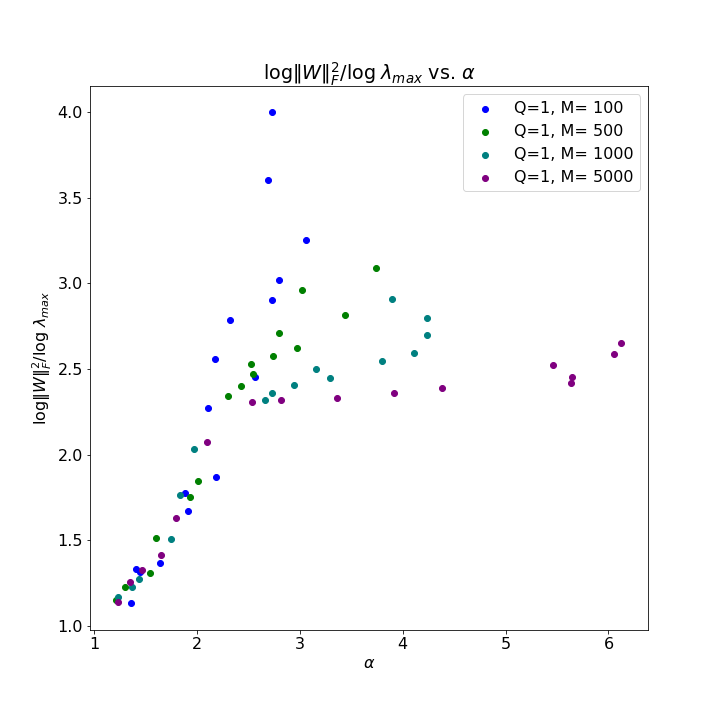
\includegraphics[scale=0.30]{img/Alpha-LogNorm-Relations.png}
%%       \label{fig:randW}
%%    }
%%    \subfigure[$\dfrac{1}{N^{2/\mu}}$ normalization] {
%%       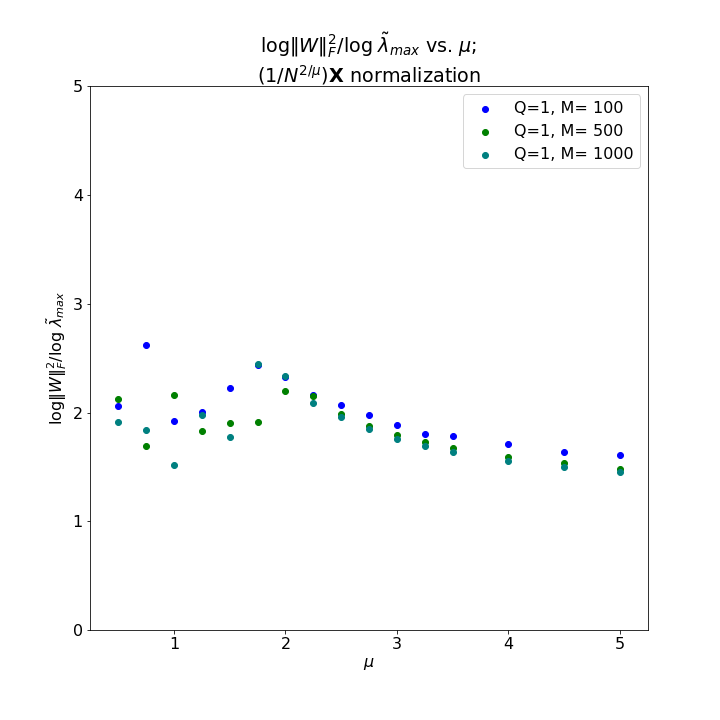
\includegraphics[scale=0.30]{img/LogNorm-Lmax-Scaled.png}
%%       \label{fig:logNormHat}
%%    }
%%    \caption{
%%             Numerical test of Eqn.~(\ref{eqn:basic_relation}) for random HT matrices; and the effect of different normalizations.
%%             \michael{Careful about $\alpha$ versus $\mu$ here.}
%%             \michael{Mention finite-size issues versus saturation.}
%%            }
%% \end{figure}
%% 
%% If, instead, we normalize the correlation matrix $\mathbf{X}$ by $N^{2/\mu}$, then we get very different behavior.
%% Let 
%% %$$
%% %\tilde{\mathbf{X}}=\dfrac{1}{N^{2/\mu}}\mathbf{W}^{T}\mathbf{W}  ,
%% %$$
%% $
%% \tilde{\mathbf{X}}=\dfrac{1}N^{-2/\mu}\mathbf{W}^{T}\mathbf{W}  ,
%% $
%% in which case we call $\tilde{\lambda}$ a \emph{scale-free eigenvalue} of $\tilde{\mathbf{X}}$, i.e.,
%% $  %$$
%% \tilde{\mathbf{X}}\mathbf{v}=\tilde{\mathbf{X}}\tilde{\lambda}  .
%% $  %$$
%% If we compute the scale-free eigenvalues, and we fit them to a PL exponent $\tilde{\alpha}$, then we find that the Frobenius norm is dominated by the maximum (scaled) eigenvalue $\tilde{\lambda}$ of $\tilde{\mathbf{X}}$.  
%% This is depicted in 
%% Figure~\ref{fig:logNormHat}
%% for our simulated Pareto matrices $\mathbf{W}^{rand}(\mu)$ which shows
%% %the log Frobenius norm squared, $\log_{10}\Vert\mathbf{W}\Vert^{2}_{F}$, divided by $\log_{10}\tilde{\lambda}$,
%% $\log\Vert\mathbf{W}\Vert^{2}_{F}/\log\tilde{\lambda}$,
%% for all for all ranges of $\mu$.
%% 
%% %%\begin{figure}[!htb]
%% %%   \centering
%% %%   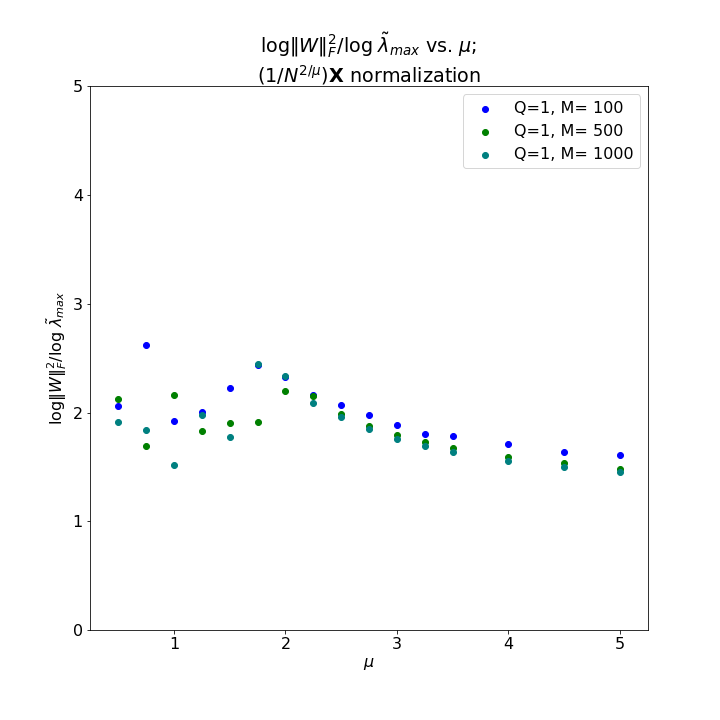
\includegraphics[scale=0.30]{img/LogNorm-Lmax-Scaled.png}
%% %%   \caption{R XXX.  WE MAY WANT THREE SUBFIGURES HERE.
%% %%   \michael{Charles suggest we don't need this figure and related discussion, decide later as text evolves.}
%% %%   }
%% %%  \label{fig:logNormHat}
%% %%\end{figure}
%% 
%% \charlesX{UGH I forgot why this is 2 .. we need to review the data and what was done and check the math carefully}\michael{Is this comment stale or still to deal with.}
%% 
%% Notice that this linear relations holds quite well, albeit with a large error bar, for $1<\mu<2$, even for small matrices, but starts to degrade for $\mu>2$.
%% This simple linear relation characterizes the scale invariant properties of the VHT Levy matrices; they are dominated by the largest scale-free eigenvalue.
%% 
%% $$\Vert\mathbf{W^{rand}(\mu)}\Vert^{2}_{F}\approx\tilde{\lambda}_{max},\;\;\mu=1$$
%% 
%% \nred{This might need to be
%% $$\Vert\mathbf{W^{rand}(\mu)}\Vert^{2}_{F}\approx\tilde{\sigma}^{2}_{max},\;\;\mu=1$$
%% }
%% 
%% which is good to within $5\%$ on a log scale
%% 
%% $$\log\;\Vert\mathbf{W^{rand}(\mu)}\Vert^{2}_{F}\approx\log\;\tilde{\lambda}_{max},\;\;1<\mu<2$$


\section{Random Pareto versus Non-random DNN Matrices} 
%\section{Heavy-Tailed Universality: Random Pareto versus Non-random DNN Matrices} 
\label{sxn:appendix-universality}

When we use Universality, as we do in our derivation of the basic PL--Norm Relation, we would like a method that applies both to HT random matrices as well as to non-random, indeed strongly-correlated, pre-trained DNN layer weight matrices that (as evidenced by their ESD properties) are in a HT Universality class.  
To accomplish this, however, requires some care: while the pre-trained $\mathbf{W}$ matrices do have ESDs that display empirical signatures of HT Universality~\cite{MM18_TR}, they are \emph{not} random Pareto matrices.
Many of their properties, including their empirical Frobenius norms, behave very differently than that of a random Pareto matrix.  
(We saw this in Figure~\ref{fig:relations}, which showed that $ \alpha\log\lambda_{max} $ achieves much larger values for HT random matrices than real DNN weight matrices.)

To illustrate this, we generate a large number of HT random matrices $\mathbf{W}^{rand}(\mu)$, with exponents $\mu\in[0.5, 5]$, as described in Section~\ref{sxn:theory-new}.
%
We then fit the ESD of each $\mathbf{W}^{rand}(\mu)$ to a PL using the method of Clauset et al.~\cite{CSN09_powerlaw,ABP14} to obtain the empirical exponent $\alpha$. 
Figure~\ref{fig:fro-rand} displays the relationship between the (log of the squared) Frobenius norm and the $\mu$ exponents for these randomly-generated Pareto matrices.
(Similar but noisier plots would arise if we plotted as a function of $\alpha$, due to imperfections in the PL fit.)
We did the same for the weight matrices (extracted from the Conv2D Feature Maps) from the pre-trained VGG11 DNN, again as described in Section~\ref{sxn:theory-new}.
Figure~\ref{fig:fro-vgg11} displays these results, here as a function of $\alpha$.
\michael{Charles, maybe plot both as a function of $\alpha$, since they are different, and consistent with text.}

\begin{figure}[!htb]
   \centering
   \subfigure[Random Pareto Matrices] {
      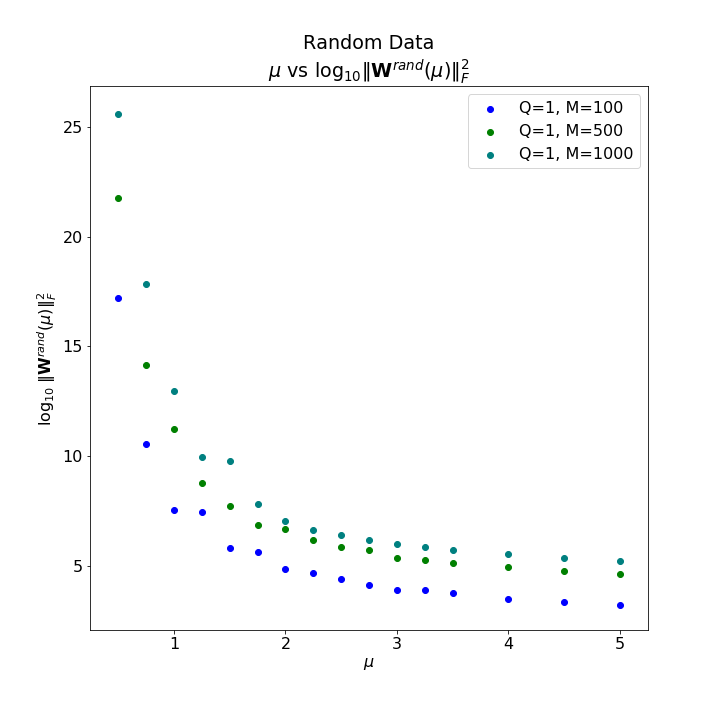
\includegraphics[scale=0.30]{img/fro-rand.png} 
      \label{fig:fro-rand}
   }
   \subfigure[Pre-trained VGG11 Weight Matrices]{
      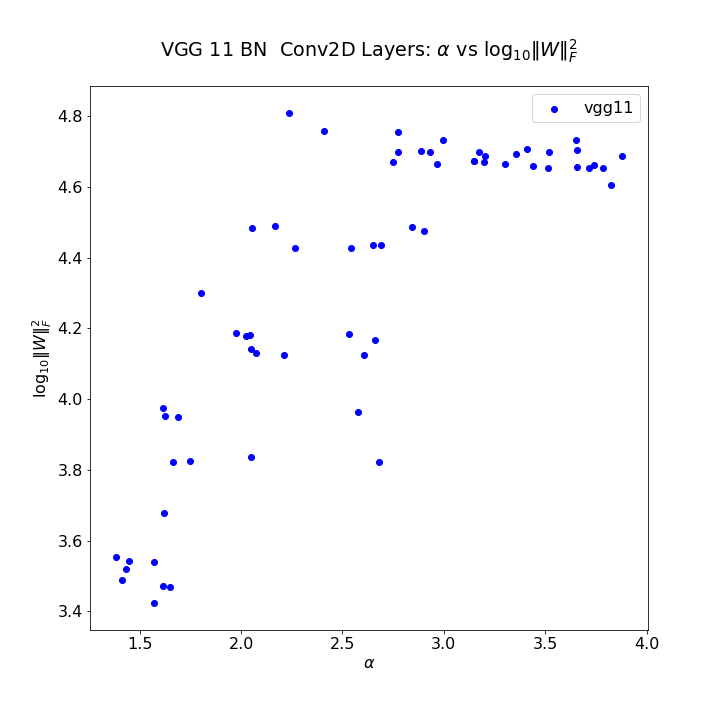
\includegraphics[scale=0.30]{img/fro-vgg11.png} 
      \label{fig:fro-vgg11}
   }
   \caption{Dependence of Frobenius norm on PL exponents for random Pareto versus pre-trained DNN matrices.  }
   \label{fig:fnorm}
\end{figure}

The properties of $\Vert\mathbf{W}\Vert^{2}_{F}$ for the random Pareto versus real/ron-random DNN weight matrices are quite different.
For a random Pareto matrix, $\mathbf{W}^{rand}(\mu)$, the Frobenius norm $\Vert\mathbf{W}^{rand}(\mu)\Vert^{2}_{F}$ 
\emph{decreases with increasing exponent} $(\mu)$; and there is a modest finite-size effect.
(In addition, as the tails of the ESD $\rho(\lambda)$ get heavier, the largest eigenvalue $\lambda_{max}$ of $\mathbf{X}$ scales with the largest element of $\mathbf{W}^{rand}(\mu)$.) 
% \michael{$\alpha$ or $\mu$ here.}
% \michael{Cite something or show this.}
For the weight matrices of a pre-trained DNN, however, the Frobenius norm $\Vert\mathbf{W}\Vert^{2}_{F}$ \emph{increases with increasing exponent} $(\alpha)$, saturating at $\alpha\approx 3$.
This happens because, due to the training process, the $\mathbf{W}$ matrices themselves are highly-correlated, and not random matrices with a single large, atypical element.
In spite of this, the ESD $\rho(\lambda)$ of these pre-trained correlations matrices $\mathbf{X}$ display Universal HT behavior~\cite{MM18_TR}; and, as shown in Figure~\ref{fig:relation-vgg11}, 
Eqn.~(\ref{eqn:basic_relation}) is approximately satisfied, in the sense that 
$\alpha\log\lambda_{max}$ is positively correlated with $\log\Vert\mathbf{W}\Vert^{2}_{F} $.
This is one of the remarkable properties of Universality (and it shows why some care must be taken in applying these Universality principles).
 

\newpage
\section{Appendix: Michael's Derivation}
\label{sxn:appendix-michael_derivation}

\michael{MM probably remove this entirely, unless relate to synthetic empirical results.}

Here, we derive an expression for the ratio of the log of the Frobenius norm of $W$ to the log of the spectral norm of $W$.
Once we settle on presentation, with normaliation, etc., this will probably be a ``subroutine'' in our analysis.
To simplify things, we will be interested in the matrix $W$, and in particular the Frobenius norm $\|W\|_F$ and spectral norm $\|W\|_2$ of this matrix.
Then, given these expressions, we will derive other things, e.g., norms of correlation matrices with different normalizations, etc., by using different normalizations.  

Recall that we are modeling the matrix $W$ as a random matrix with heavy-tailed entries.
XXX.  WE MIGHT WANT A FIGURE SHOWING THE REAL DATA LOOKS LIKE THIS, LIKE THE BURDA PAPER.
Thus, the Frobenius norm is going to be related to the second moment of the entries, and the spectral norm is going to be related to the largest entry.
XXX.  CITE AUFFINGER PAPER FOR EXACTLY THE RANGE OF VALIDITY OF THIS.
An important issue will be the power law exponent, since---depending on it---familiar results will hold or will fail to hold.
For the moment, let's ignore that we are dealing with matrices, and let's focus on drawing elements from a heavy-tailed distribution, and computing various moments and extreme values of empirical draws.

Consider the extreme case of a HT distribution, namely a PL distribution.
XXX.  INCLUDE SOMETHING ABOUT SLOWLY VARYING FUNCTION AS WELL AS XMIN VALUE.
Up to a slowly-varying function, the general form of the probability distribution function is
$$
p(x) = \frac{C}{x^{1+\mu}}  = C x^{-1-\mu} , 
$$
where $\mu > -1$, and where $x \in [x_{min},\infty)$.
The cdf 
XXX ACTUALLY ONE MINUS THAT 
is then
$$
P_{\ge}(x) = \int_x^{\infty} p(x^{\prime}) dx^{\prime} 
           = \frac{C}{\mu} \frac{1}{x^{\mu}}  
           = \frac{C}{\mu} x^{-\mu}  .
$$
In order to compute $C$ and normalize these expressions, let
\begin{eqnarray*}
1 = \int_{x_{min}}^{\infty} p(x) dx 
  = C \int_{x_{min}}^{\infty} x^{-1-\mu} dx 
  = \frac{C}{-\mu} x^{-\mu} |_{x_{min}}^{\infty}  
  = \frac{C}{\mu} x_{min}^{-\mu}   ,
\end{eqnarray*}
which is valid (i.e., the integral converges and exists) if $\mu > 0$.
From this, is follows that the normalization constant is
\begin{equation}
C = \mu x_{min}^{\mu}  .
\label{eqn:pl_normalization}
\end{equation}
Thus, if $\mu > 0$, then the probability distribution function is 
\begin{equation}
p(x) 
%     = \frac{\mu}{x_{min}}\left( \frac{x_{min}}{x}\right)^{1+\mu}  
     = \frac{\mu}{x_{min}}\left( \frac{x}{x_{min}}\right)^{-1-\mu}  ,
\label{eqn:pl_pdf}
\end{equation}
and the cdf 
XXX ACTUALLY ONE MINUS THAT
is 
\begin{equation}
P_{\ge}(x) 
%           = \left( \frac{x_{min}}{x} \right)^{\mu}  
           = \left( \frac{x}{x_{min}} \right)^{-\mu}  .
\label{eqn:pl_one_minus_cdf}
\end{equation}
XXX.  MENTION SLOWLY VARYING THING, MAYBE AS CLAUSET DID.

An important aspect of heavy-tailed probability distributions is that extreme values, i.e., values very far from the mean (when the mean is even defined) are not extremely uncommon (as they are for distributions in the Gaussian universality class).
Of particular relevance for us is the largest value $x_{max}$ obtained when sampling from Eqn.~(\ref{eqn:pl_pdf}) in $n$ i.i.d. trials.
It is known, see e.g.~\cite{SornetteBook,BouchaudPotters03,newman2005_zipf}, that the expectation of $x_{max}$ for $\mu\in(1,2)$ 
XXX IS THIS TRUE FOR MORE GENERAL PL PARAMETERS
is given~by:
$$
\ExpectBracket{x_{max}} \approx x_{min} n^{1/\mu}  .
$$

Let's return to the expression given in Eqn.~(\ref{eqn:pl_pdf}) and compute the first few moments of this distribution.
The first moment is
\begin{eqnarray*}
\ExpectBracket{x} = \int_{x_{min}}^{\infty} x p(x) dx  
                  = C \int_{x_{min}}^{\infty} x^{-\mu} dx 
                  = \frac{C}{1-\mu} x^{1-\mu} |_{x_{min}}^{\infty} 
                  = \frac{\mu}{\mu-1} x_{min}    ,
\end{eqnarray*}
which is valid if $\mu > 1$.
Similarly, the second moment is
\begin{eqnarray*}
\ExpectBracket{x^2} = \int_{x_{min}}^{\infty} x^2 p(x) dx  
                    = C \int_{x_{min}}^{\infty} x^{1-\mu} dx 
                    = \frac{C}{2-\mu} x^{2-\mu} |_{x_{min}}^{\infty} 
                    = \frac{\mu}{\mu-2} x_{min}^2  ,  
\end{eqnarray*}
which is valid if $\mu > 2$.
While this second moment expression is valid for $\mu > 2$, we are going to want a similar expression for $\mu \in (1,2)$.
For this we can integrate up to $x_{max}$, rather than up to $\infty$.
In more detail, for $\mu \in (1,2)$, the empirical second moment is
\begin{eqnarray*}
\ExpectBracket{x^2} &=&       \int_{x_{min}}^{x_{max}} x^2 p(x) dx  \\
                    &=&       \frac{C}{2-\mu} x^{2-\mu} |_{x_{min}}^{x_{max}}  \\
                    &\approx& \frac{\mu}{2-\mu} x_{min}^{\mu} \left( x_{min}^{2-\mu} n^{(2-\mu)/\mu} - x_{min}^{2-\mu} \right) \\
                    &\approx& \frac{\mu}{2-\mu} x_{min}^{2} n^{(2-\mu)/\mu}   ,
\end{eqnarray*}
which is valid for $\mu\in(1,2)$.
Note that in these expressions and the expressions below, we follow previous work \cite{MM18_TR} and don't compute expressions for $\mu=2$ precisely.
(They are known to lie in yet another universality class~\cite{SornetteBook,BouchaudPotters03}, and we don't expect to resolve the difference numerically.)

Finally, consider an $N \times N$ matrix $W$. 
Then, 
$\|W\|_2 = w_{min} N^{2/\mu}$ (for $\mu\in(1,2)$) and
$\|W\|_2 = w_{min} N^{1/2}$ (for $\mu>2$).
XXX.  CHECK THAT I AM NOT OFF By A FACTOR OF N.
Thus, for the spectral norm, we have that: 
\begin{equation}
\|W\|_2^2 = \left\{ \begin{array}{ll}
                       w_{min}^2 N^{4/\mu} & \mbox{if $\mu\in(1,2)$} \\
                       w_{min}^2 N & \mbox{if $\mu > 2$} (XXX CHECK)
                    \end{array}
            \right.
\end{equation}
Similarly, for the Frobenius norm, we have that:
\begin{equation}
\|W\|_F^2 = \left\{ \begin{array}{ll}
                      \frac{\mu}{2-\mu} w_{min}^2 N^{(4-2\mu)/\mu} & \mbox{if $\mu\in(1,2)$} \\
                      \frac{\mu}{\mu-2} w_{min}^2 N^2 & \mbox{if $\mu > 2$} 
                    \end{array}
            \right.
\end{equation}

We are interested in the function of $\mu$ defined as:
$$
f = f(\mu) = \frac{\log \|W\|_F^2}{\log \|W\|_2^2}  .
$$
From the above, if we take logs, then for $\mu\in(1,0)$, we get:
$$
f(\mu) = \frac{ \log\left(\frac{\mu}{2-\mu}\right) + \log(w_{min}^2) + \frac{4}{\mu}\log N - 2 \log N }{ \log(w_{min}^2) + \frac{4}{\mu}\log N }
$$
and for $\mu > 2$, we get:
$$
f(\mu) = \frac{ \log\left(\frac{\mu}{\mu-2}\right) + \log(w_{min}^2) + 2 \log N }{ \log(w_{min}^2) + \log N }
$$


% \section{Appendix: Refs: MM TO INCORPORATE THESE INTO TEXT}
% 
% Our theory of Implicit Self Regularization used Heavy Tailed Random Matrix Theory (HT RMT), and here we use HT RMT also~\cite{MM18_TR}.
% See also our prior results on \cite{MM17_TR}.
% 
% \cite{NTS14_TR} is 
% Neyshabur et al. on :
% ``In search of the real inductive bias: on the role of implicit regularization in deep learning''
% 
% \cite{NTS15} is
% Neyshabur et al. on:
% ``Norm-Based Capacity Control in Neural Network''
% 
% \cite{NBMS17_TR} is 
% Neyshabur et al. on:
% ``Exploring generalization in deep learning''
% 
% \cite{AGNZ18_TR} is 
% Arora et al. on:
% ``Stronger generalization bounds for deep nets via a compression approach''
% 
% \cite{ACH18_TR} is 
% Arora et al. on:
% ``On the Optimization of Deep Networks: Implicit Acceleration by Overparameterization''
% 
% \cite{Bar97} is
% Bartlett on:
% ``For valid generalization, the size of the weights is more important than the size of the network''
% 
% \cite{BFT17_TR} is 
% Bartlett et al. on:
% ``Spectrally-normalized margin bounds for neural networks''
% 
% \cite{SHNx17_TR} is 
% Soudry et al. on: 
% ``The implicit bias of gradient descent on separable data''
% 
% \cite{YM17_TR} is 
% Yoshida and Miyato on:
% ``Spectral norm regularization for improving the generalizability of deep learning''
% 
% \cite{LMBx18_TR} is 
% Liao et al. on:
% ``A surprising linear relationship predicts test performance in deep networks''
% 
% \cite{PLMx18_TR}
% is Poggio el at. on: 
% ``Theory {IIIb}: Generalization in Deep Networks''
% 
% \cite{KKB17_TR} is 
% Kawaguchi et al. on:
% ``Generalization in Deep Learning''
% 
% \cite{NBS17_TR} is:
% Neyshabur et al. on: 
% ``A {PAC}-{B}ayesian Approach to Spectrally-Normalized Margin Bounds for Neural Networks''
% 
% \cite{ZF18_TR} is
% Zhou and Feng on:
% ``Understanding Generalization and Optimization Performance of Deep {CNN}s''
% 
% \cite{BJNx01_TR} is
% Burda et al. on:
% ``{L}{\'e}vy Matrices and Financial Covariances''
% 
% \cite{MN09_TR} is
% Mahoney and Narayanan on:
% ``Learning with Spectral Kernels and Heavy-Tailed Data''
 

